 \section{Belief Propagation Decoding for 2 User Gaussign MAC}
 The mathematical model of 2 user Gaussign Multiple Access channel is given in Figure~\ref{fig:awgn_channel}. The capacity region is given by
 \begin{eqnarray}
  R^{[1]} &\leq& I(X_1;Y|X_2) \nonumber \\
  R^{[2]} &\leq& I(X_2;Y|X_1) \nonumber \\
  R^{[1]} + R^{[2]} &\leq& I(X_1, X_2;Y) \nonumber
 \end{eqnarray}
The capcity region looks like the curve shown in Figure~\ref{fig:awgn_channel_capacity}. We are intereseted in the rate pairs on the 
dominant face $\mathcal{D}$ of the capacity region for the points on $\mathcal{D}$ gives the maximum sum rate. The corner points are
achievable by successive decoding. The other pointes are achieved through rate splitting or time sharing. Here we present joing decoding
of the two users using belief propogation to achieve a general point on $\mathcal{D}$ without rate splitting or time sharing.
To decode $x_i^{[i]}$, the $i^{th}$ bit of user 1, we have the following MAP decoding rule.
\begin{eqnarray}
 \hat{x}_i^{[1]} 	&\overset{\Delta}{=}& \text{arg} \max_{x_i}p_{X_i^{[1]}|Y}(x_i^{[1]}|y) \\
			&=& \text{arg} \max_{x_i}\sum_{\sim x_i^{[1]}}p_{X^{[1]}, X^{[2]}|Y}(x^{[1]}, {x^{[2]}|y) \\
			&=
\end{eqnarray}

 \begin{figure}[scale=1, !tp]
 \centering
  \begin{tikzpicture}
  \draw (0, 0) node[circle, thick, draw] (f) {$+$};
  \path [draw, latex] (-3, -1) -- node[near start, below]{$X_i^{[2]}$} (-1, -1) ;
  \path [draw, latex] (-3, 1) -- node[near start, below]{$X_i^{[1]}$} (-1, 1) ;
  \path [draw, -latex] (-1, -1) -- (f) ;
  \path [draw, -latex] (-1, 1) -- (f) ;  
  \path [draw, -latex] (f) -- node[near end, below]{$Y_i$}(2, 0) ;
  \path [draw, -latex] (0, -2) -- (f);
  \draw (0, -2.3) node{$Z_i \sim \mathcal{N}(0, \sigma^2)$};
   \end{tikzpicture}
\caption{AWGN Multiple Access Channel}
\label{fig:awgn_channel}
\end{figure}


\begin{figure}[scale=1, !tp]
 \centering
  \begin{tikzpicture}
  \path [draw, thick, -latex] (0, 0) -- node[at end, left]{$R^{[2]}$} (0, 5) ;
  \path [draw, thick, -latex] (0, 0) -- node[at end, above]{$R^{[1]}$} (5, 0) ;
  \path [draw, latex] (0, 4) -- (2, 4) ;
  \path [draw, latex] (4, 0) -- (4, 2) ;
  \path [draw, latex] (2, 4) -- (4, 2);
  \draw [dotted, thick] (2, 4) -- (2, 0);
  \draw [dotted, thick] (4, 2) -- (0, 2);
  \draw (-0.75, 2) node{$I(X_2;Y)$};
  \draw (2, -0.25) node{$I(X_1;Y)$};
  \draw (-1, 4) node{$I(X_2;Y|X_1)$};
  \draw (4, -0.25) node{$I(X_1;Y|X_2)$};
  \end{tikzpicture}
\caption{Capacity of AWGN Multiple Access Channel}
\label{fig:awgn_channel_capacity}
\end{figure}

\begin{figure}
 \centering
 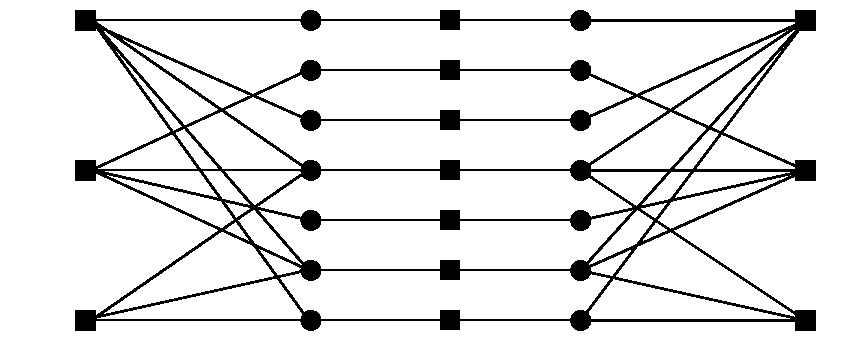
\includegraphics[scale=1]{2user.pdf}
\end{figure}
